\documentclass{article}

% Packages
\usepackage{amsmath} % For mathematical symbols and equations
\usepackage{graphicx} % For including images
\usepackage{cite} % For managing citations
\usepackage{lipsum} % For generating dummy text
\usepackage{algorithm} % For writing algorithms
\usepackage{algpseudocode} % For writing pseudocode
\usepackage[a4paper, total={6in, 8in}]{geometry}
\usepackage{hyperref} % For hyperlinks

% Title and Author
\title{Engineering Algorithms for Large Network Applications}
\author{Abhishta G. Adyatma}
\date{}

\begin{document}

\maketitle

\section{Introduction}

Large networks are characterized as $G = (V, E)$ where there exists an abundant amount of Vertices (V) and Edges (E).
These networks are often used to model real-world structures like roads, railways, air traffic, and social networks.
Traversing these vast networks poses a significant challenge, particularly when dealing with millions of vertices and edges.
Within this report, the author delves into several approaches aimed at efficiently solving single-source single-target query
(shortest path problems) with reducing the search space (number of vertices visited) of the Dijkstra's Algorithm.

As discussed in \cite{Zaroliagis2008}, the resolution of single-source single-target path problems on expansive 
networks typically revolves around two primary approaches. The first method, termed 'Graph Annotation,' involves 
adding supplementary information to the vertices and/or edges within the graph. This information facilitates 
acceleration techniques aimed at discerning which vertices require no further exploration. Variants of this 
approach may encompass heuristic computations aimed at estimating vertex distances. Additionally, certain variations
involve pre-computations that establish constraints and enable the pruning of vertices during the search process \cite{Wagner2005}.

The second approach, termed 'Auxiliary Graph' involves the construction of a secondary graph from 
the original graph to aid in solving specific problems or performing certain operations more efficiently.
Auxiliary graphs simplify complex problems, enable efficient algorithmic solutions, or provide alternative 
representations for specific analyses. Variants of this approach may encompass the construction of an 
\textit{Overlay Graph} \cite{Holzer2008}, Spanning Trees, or using methods of Graph Aggregations \cite{Sieranoja2022} to fabricate
a higher-level abstraction.

This report aims to conduct a benchmarking analysis of multiple approaches 
using a large network dataset. The goal is to delve into the performance and constraints of previously introduced approaches and their algorithm implementations. The author's focus 
will be on key metrics, including the Average Visits (number of vertices visited), Average Query Time (time taken to solve a shortest-path problem), and in selected implementations, the Average Resolution Time (time taken to complete a single vertex computation).

\section{Dataset}

In this report's experimentation, the author chose to benchmark the algorithms using the \href{http://www.diag.uniroma1.it/~challenge9/download.shtml}{9th DIMACS Implementation Challenge - Shortest Paths}. This dataset provides 12 representations of the USA road networks. The primary focus of this report is on two specific networks: the New York Road Network, comprising 264,346 vertices and 733,846 edges, and the San Francisco Bay Area Road Network, containing 321,270 vertices and 800,172 edges. Three files are mainly found on each dataset, the Distance, the Time, and the Coordinate of each edges and vertices. The author will focus on the Distance information for benchmarking.

Additionally, to facilitate memory-intensive pre-computations and/or run-times required by certain algorithms, the author created subset variations of each road network of 50,000 and 10,000 edges. These information are displayed in Table \ref{tab:datacomp}.


\begin{table}
    \centering
    \begin{tabular}{ccc}
        Dataset & Num. Vertices & Num. Edges \\
        \hline
        NY & 264,346 & 733,846 \\
        NY (50K) & 20,386 & 50,000 \\
        NY (10K) & 4,154 & 10,000 \\
        \hline
        BAY & 321,270 & 800,172 \\
        BAY (50K) & 18,322 & 50,000 \\
        BAY (10K) & 4,164 & 10,000 \\
        \hline
    \end{tabular}
    \caption{Dataset Composition}
    \label{tab:datacomp}
\end{table}

\section{Algorithms}

The author experimented with several algorithms specific to Graph Annotation and Auxiliary Graph approaches aimed at minimizing the Average Visits and Average Query Time of the baseline algorithm. The author chose Dijkstra's Algorithm to be the best line since there were no negative weights in the experimented dataset. The following comparison algorithm shows a variety of approaches from Heuristics (Approximation), Graph Annotation through Containerization of Vertices, and Minimizing the Graph through an Auxiliary Graph. 

\subsection{Dijkstra (Baseline)}

Dijkstra's algorithm serves as the baseline of this analysis. It's 
implemented in a single-source, single-target setup, designed to conclude 
the search once the target vertex has been visited. This particular 
implementation employs a Binary Heap Min Priority Queue, offering a time 
complexity of \(O(E \ log \ V)\). Overall, the goal of the next few 
implementations are to reduce the baseline search space (Average Visits).

\subsection{A* Haversine Distance}

\begin{algorithm}
\caption{Relaxation with Haversine Distance Heuristic}\label{alg:cap}
\begin{algorithmic}
\Function{Relax}{u, v, e, w, H}
   \If{$d[v] > d[u] + w(u, v) + H(v, e)$}
    \State $d[v] = d[u] + w(u, v) + H(v, e)$ \Comment{H is the Haversine Formula, e is the End Vertex}
   \EndIf
\EndFunction
\end{algorithmic}
\label{algorithm:relaxH}
\end{algorithm}

Given the dataset has information on the vertex geographic coordinates,
the author pursues an approach to construct a heuristic that estimates the
neighboring vertex against the end vertex during the search. These additional information supplemented to the vertices enters the approach of Graph Annotation where it can make calculations to extend the baseline algorithm further. To approximate the distance between neighboring vertex and end vertex, the Haversine Formula (defined by Equation \ref{hav} \& \ref{havD}) is used on both geographic coordinates. 

\begin{equation}
    hav(\theta) = \sin^2\left(\frac{\Delta\text{lat}}{2}\right) + \cos(\text{lat}_1) \cdot \cos(\text{lat}_2) \cdot \sin^2\left(\frac{\Delta\text{lon}}{2}\right)
\label{hav}
\end{equation}

\begin{equation}
    distance = 2 \cdot R \cdot \text{atan2}\left(\sqrt{hav(\theta)}, \sqrt{1 - hav(\theta)}\right)
\label{havD}
\end{equation}

This approximation is reliable for every calculation within the experimented dataset because the weight function correlates with the Haversine Distance, giving the algorithm clear approximations between the source and the target. Moreover, Algorithm \ref{algorithm:relaxH} shows a modified `RELAX` function with 
addition of the heuristic of `H(v, e)` which calculates the distance. `H(v, 
e)` will continuously be smaller if the neighboring vertex is closing in to 
the end vertex. Intuitively, this will decrease the Average Visits per Query
with this additional information being calculated. Additionally, the 
computation of this heuristic have a time complexity of \(O(1)\) which with Dijkstra's Algorithm implementation remains $O(E \ log \ V)$.

\subsection{Geometric Containers}

The approach explored by \cite{Wagner2005} focuses on minimizing the search 
space further through methods of pre-computations. This method involves constructing a 
`container,` which comprises of sets of vertices strategically chosen to 
enhance efficiency in subsequent shortest-path computations. In Figure \ref{fig:geoconstruct}, the algorithm iterates over all vertices to enlarge $C(u, v)$ with vertex encountered from the single-source of $s$. This will include all vertices visited from $s$ to $v$ to enter the container.

\begin{figure}[b!]
    \centering
    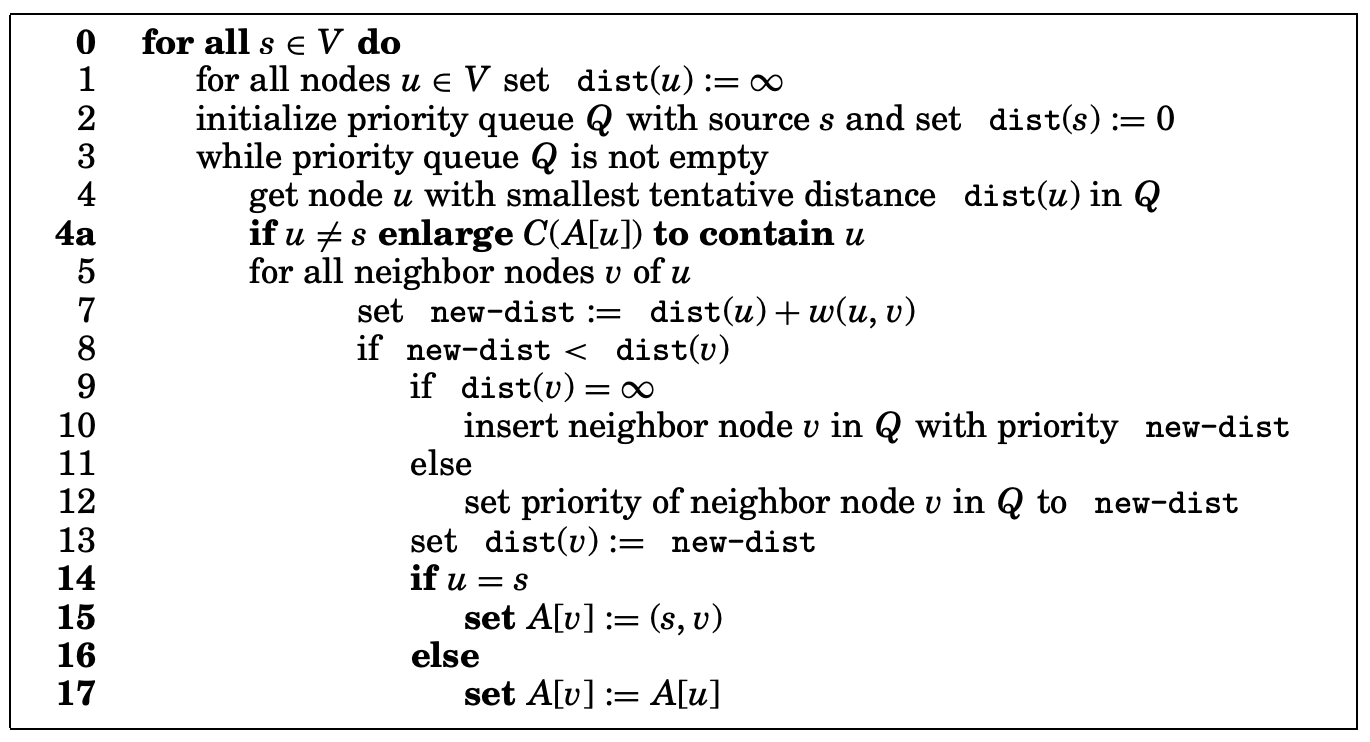
\includegraphics[width=0.7\linewidth]{img/container.png}
    \caption{Geometric Container Construction (Wagner et al., 2005)}
    \label{fig:geoconstruct}
\end{figure}

These containers play a pivotal role in restricting the search space of Dijkstra's algorithm, this is referred as `Dijkstra Pruning`, depicted in Figure \ref{fig:geodijkstra}. This adaptation of Dijkstra's method integrates the pre-computed containers. Specifically, if the end vertex \(t\) belongs to \(C(u,v)\), then the algorithm navigates to vertex \(v\). The success of this algorithm heavily hinges on the quality of the containers, which can fluctuate in size relative to the graph.

\begin{figure}
    \centering
    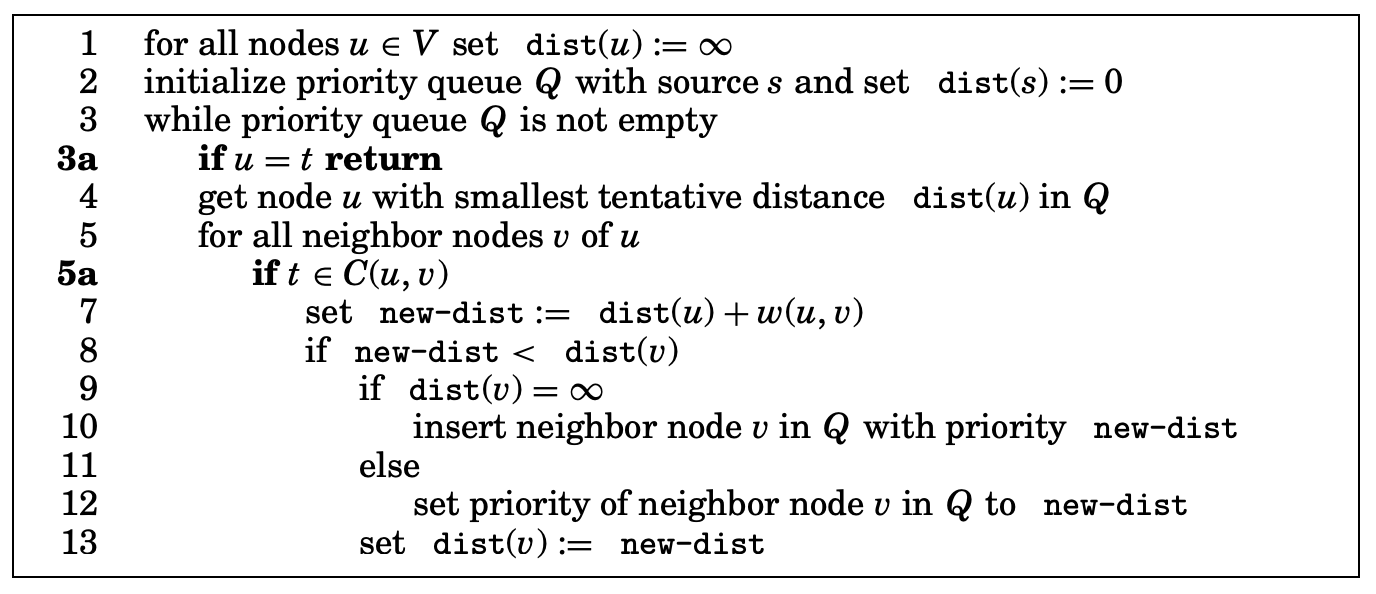
\includegraphics[width=0.7\linewidth]{img/pruning.png}
    \caption{Dijkstra with Pruning (Wagner et al., 2005)}
    \label{fig:geodijkstra}
\end{figure}

Moreover, this algorithm falls into the category of approach of Graph Annotation since it is supplying additional information between edges. Further analyzing the algorithms complexity, constructing the containers takes a time complexity of $O((E \ log \ V) * V)$ with a space complexity stated to be $O(E * V)$. This is due to computing for all vertices. As for the search algorithm, the time complexity remains $O(E \ log \ V)$.

\subsection{Min Overlay Graph}

Constructing an Overlay Graph, defined as a graph $G = (V,E$) on a subset $S \subseteq V$ is a graph with vertex set $S$ and edges corresponding to shortest paths in $G$ \cite{Holzer2008}, would create a representation
of the original Graph with a selection of vertices and edges that is minimal
to all-pairs within $S$. This type of approach is an example of an Auxiliary Graph approach, where a secondary graph is constructed to either
aid or solve the problem entirely.

\begin{figure}
    \centering
    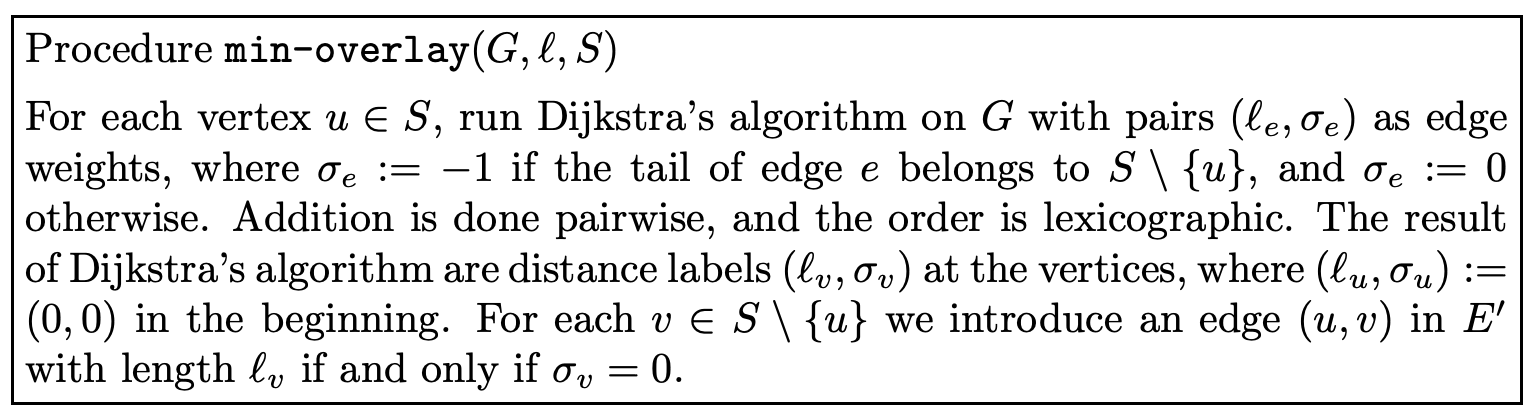
\includegraphics[width=0.7\linewidth]{img/minoverlay.png}
    \caption{Min Overlay Procedure (Holzer et al., 2008)}
    \label{fig:minoverlay}
\end{figure}

Figure \ref{fig:minoverlay} illustrates the construction process of the Min Overlay Graph. This method leverages a customized version of the Dijkstra Algorithm, incorporating adjustments to handle pairs of $(\ell_e, \sigma_e)$. These pairs guide the algorithm's decision-making during the search phase to determine whether a specific vertex should be included in the set of edges \(E'\) connected to vertex \(u\) or not. Specifically, the value of \(\sigma\) is modified to \( -1 \) selectively during the exploration process when the algorithm encounters a current vertex \(c \in V\) and a neighboring vertex \(n \notin S\).

With this algorithm, constructing a Min Overlay Graph would have a time complexity of $O((E \ log \ V) * S)$. However, this report's implementation towards this approach only explores the construction of the Min Overlay Graph such that any query $v \in S$ has a time complexity of $O(1)$. Looking at variations of similar implementations, this algorithm can also be paired with Dijkstra to search a shortest-path between two vertices where $(u,v) \notin S$. Ultimately, this algorithm can speed up a shortest-path problem partially if $S \subset V$ else then Dijkstra with a Min Overlay Prioritization can aid to reduce the search space.

\section{Experimental Results}

\subsection{Setup}

For this report's experimentation, the author analyzes the aforementioned algorithms using an Apple M1 Chip with 8 GB Memory. All algorithm implementations are using Go 1.18+ with base implementations (no external libraries are used). The scope of analysis this report could achieve is bounded to this hardware specification. The experiment is conducted on 6 Benchmarks randomly created to form a Test Case of 5000 Shortest-Path Problems each. Source code can be found at \href{https://github.com/abhishtagatya/graf}{Github : abhihtagatya/graf}

\subsection{Average Visits and Query Time}

The author's objective to reduce the number of visited nodes per query, which represents a single shortest-path problem is woven into the design of almost all the aforementioned algorithms. The total number of visits and query time per test set iteration are aggregated and subsequently averaged across the benchmark set's size to derive meaningful metrics. The algorithms considered for this metric includes the Dijkstra (Original Implementation), Dijkstra (Baseline), A* Haversine, and the Geometric Container algorithms.

\begin{table}
    \centering
    \begin{tabular}{ccccccccc}
 & \multicolumn{2}{c}{Dijkstra (Original)}& \multicolumn{2}{c}{Dijkstra (Baseline)}& \multicolumn{2}{c}{A* Haversine}& \multicolumn{2}{c}{Geo. Container}\\
 \hline
         &  Visit&  Time&  Visit&  Time&  Visit&  Time&  Visit& Time\\
         \hline
         NY&  264,346&  277.19ms&  131,828&  132.87ms&  \textbf{29,195}&  \textbf{47.6ms} &  -& -\\
         NY (50K)&  9,346&  5.69ms&  6,737 &  4.04ms&  5,277&  5.5ms&  \textbf{52}& \textbf{2.57ms}\\
         NY (10K)&  3,682&  2.17ms&  1,934&  1.12ms&  684&  651.68µs&  \textbf{44}& \textbf{435.56µs}\\
         \hline
         BAY&  321,270&  313.8ms&  160,431&  155.2ms&  \textbf{82,375}&  \textbf{129.64ms}&  -& -\\
         BAY (50K)&  10,880&  7.61ms&  6,824&  4.87ms&  4,961&  5.9ms&  \textbf{62}& \textbf{3.31ms}\\
         BAY (10K)&  482&  323.86µs&  425&  258.31µs&  398&  345.546µs&  \textbf{3}& \textbf{17.5µs}\\
         \hline
    \end{tabular}
    \caption{Average Visits and Query Time in 5000 Benchmark Sets}
    \label{tab:avgvq}
\end{table}

Table \ref{tab:avgvq} displays the performance of each algorithm to perform in each benchmark sets. The author also includes the original implementation of Dijkstra's algorithm compared to the baseline implementation of single-source single-target Dijkstra's algorithm to visualize the how a single visit to the target vertex can conclude the minimal cost between a source vertex and a target vertex.

Comparing the baseline with the A* Haversine algorithm displays that the applied heuristics to estimate the cost between a neighboring vertex to the end vertex can improve the algorithm further by $\sim41\%$. However, there has been cases recorded that shows the Average Query Time on A* Haversine algorithm is slightly higher than the baseline even though the search space is reduced. Hypothesis towards this might be due to cases where a shortest-path is not found (therefore has a distance of $\infty$) and thus the trying to compensate by finding unnecessary vertex.

The Geometric Container algorithm has reduced the search space significantly with a reduction of $\sim99\%$ compared to the A* Haversine algorithm. However, this algorithm comes with a heavy pre-computation to be able to be optimized for a specific graph. Unfortunately, this experimental setup is not capable of computing the containers for the New York Road Network and San Francisco Bay Area Road Network. Using this experimental setup, it is estimated to pre-compute both dataset with a computation time of over $\sim73$ Days with around $~16$ GB which is 4,776x the size of the original graph. Additionally, it is stated in \cite{Wagner2005}, that a change of weight or minor changes to layout might require an update on the pre-computed containers which shows the limitation of this algorithm.

\subsection{Average Resolution Time}

The author's objective to reduce the number of visited nodes per query can also be achieved through methods that does not follow searching iteratively. Through the auxiliary graph approach, it leverages methods that computes the problem (whether entirely or a subset) to create a subgraph that answers queries given some pre-computations. An example of that implementation is the Min Overlay Graph, which creates an overlay graph with all edges being the shortest-path to each. To measure the performance of this algorithm, a metric of Average Resolution Time is introduced where a Resolution Time is the time taken to resolve all queries for a single vertex $u \in S$.


\begin{table}
    \centering
    \begin{tabular}{cc}
 &Min. Overlay\\
 \hline
         & Time\\
          \hline
         NY& 14.13s\\
         NY (50K)& 576.45ms\\
         NY (10K)& 68.57ms\\
          \hline
         BAY& 14.19s\\
         BAY (50K)& 659.8ms\\
         BAY (10K)& 19.68ms\\
          \hline
    \end{tabular}
    \caption{Average Resolution Time in 5000 Benchmark Sets}
    \label{tab:avgres}
\end{table}


\section{Conclusion}

In the pursuit of forming solutions for large network applications, both approaches of Graph Annotation and Auxiliary Graph underwent extensive exploration and evaluation within the 9th DIMACS Implementation Challenge of Shortest-Paths Dataset. The findings revealed an interesting discovery: achieving a significant reduction in search space necessitates computationally intensive algorithms and pre-computations. This is clearly demonstrated in the implementation of Geometric Containers, where the trade-off between computational expense and reduced search space is discussed. Moreover, the usability of heuristics is illuminated through the A* Haversine algorithm, emerging as the least computationally demanding method while still significantly reducing the search space. Another method explored was creating a minimal subset representation of the original graph. This concept is exemplified by the implementation of the Min Overlay Graph.

Given the increasing demand for optimized algorithms in handling vast networks, future works in this realm might delve into hybrid implementations of previously studied methodologies or experiment with stacking these implementations and/or heuristics.

\bibliographystyle{plain} % Choose a style
\bibliography{references} % Assuming your file is named 'references.bib'

\end{document}
